\documentclass[twocolumn]{article}
\usepackage[english]{babel}
\usepackage[a4paper,top=2cm,bottom=2cm,left=2cm,right=2cm,marginparwidth=1.25cm]{geometry}
\usepackage{amsmath}
\usepackage{graphicx}
\usepackage{caption}
\usepackage{subcaption}
\usepackage{float}
\usepackage{multirow}
\usepackage[colorlinks=true, allcolors=blue]{hyperref}

\title{\textbf{Orange:A Novel Lens on Aging and Disease Interplay}}
\author{}
\date{\today}

\begin{document}
\maketitle

\section{Methodology}

We utilized a dataset of approximately 56,200 gene expression TPMs from 14 distinct tissue types collected from 980 subjects, sourced from the Adult Genotype-Tissue Expression (GTEx) project. \cite{gtex_bulk_expression} This dataset includes associated metadata, such as age range and circumstances of death characterized by the Hardy Scale. \cite{gtex_metadata}

Initial analysis involved generating t-SNE plots of the tissue-specific TPM values, resulting in distinct clustering of TPMs corresponding to individual tissues ...(17,000+ samples x 56,000 TPMs).... Based on these observations (Figure \ref{fig:t-SNE plots of the tissue-specific TPM values}), we selected a subset of 14 for subsequent predictive modeling of age. \\

Subsequently, we plotted t-SNE plots for the tissue samples for individual organs and observed no distinct clustering based on age range. However, in certain cases, clustering was evident when categorized by the Hardy Scale ratings. (Figure \ref{fig:T-SNE plots for individual organs_part1}) \\

Inspired by the findings in OrganAge \cite{organage2023} , we aimed to explore the potential of predicting age through the application of machine learning models.\\

\begin{itemize}
    \item Since the GTEx ... dataset does not contain every samples of every tissue type from each test subject, and neither does the aging of each organ had a strong correlation with mortality, we had to limit our study to a set of tissues that had a significant number of samples, and are known to be correlated with mortality. \cite{cdc_data_brief_2023} \cite{seer_common_cancers_2024}

    \item To develop tissue-specific aging models, we grouped the TPM data by tissue type, and then performed all training and testing on organ-specific data only. We partitioned each tissue's dataset into training and testing subsets, ensuring that all samples with a Hardy Scale rating of 1 were allocated to the testing sets. The remaining samples were randomly shuffled in a way that attempted to homogenize the distribution of death circumstance classes. To compensate for the small size of the dataset, we selected 5 percent of the shuffled samples from each organ to perform Leave-P-Out train-test splitting in a sliding window mechanism that covered each sample in the organ's dataset. Each 5 percent window was taken as the testing set, on which predictions were performed by training on the rest of the samples. This enabled us to perform a prediction on every single sample and ultimately have a larger set of predicted age-gaps, on which we could perform better downstream analyses. The samples with Hardy Scale ratings of 1, that we had initially separated for testing only, were appended to the last testing window of each tissue's dataset. We ran 25 cycles of this Leave-P-Out train test mechanism, by varying a random seed each time that affected only the initial shuffling that we performed to ensure class homogeneity.

    \item For the prediction models, we opted to employ 20x bootstrapped \textbf{Partial Least Squares (PLS) Regression} predictors to mitigate overfitting in this high-dimensional dataset. The PLS approach greatly reduces the dimensionality of the dataset and performs much faster than the Ordinary Least Squares (OLS) regressors Lasso, Ridge, and Elastic Net which employ L1 and L2 regularization. PLS regression offered the best balance between the optimization of performance metrics and the optimization of training speed. It also achieved competitive performance without the use of cross-validation in training, without which the OLS regressors could not perform so well.

    \item To further reduce noise in the dataset prior to training, we conducted a correlation analysis on the columns of TPM values for each organ. We selected only those columns exhibiting a Pearson correlation greater than 0.2, thereby retaining features that demonstrate a significant linear relationship.

    \item To compensate for the absence of precise age of the subjects in the dataset, we opted to find optimal points within each age range using simulated annealing, rather than just taking the midpoint of each range. As expected from a Gaussian distribution, the optimal point for each age range deviated from the range mid-values towards the population mean. Subsequently, utilizing the selected columns for each organ, along with sex (encoded as 0/1) and the optimal fixed point within each age range from the age column as target variables, we trained PLS predictors. The results were averaged through bootstrap aggregation to enhance model robustness and improve predictive accuracy.

    \item Following the methodology outlined in
    \textbf{OrganAge}, we employed a locally weighted scatterplot smoothing \textbf{\textit{(LOWESS)}} regression to analyze the predicted ages generated by the bootstrapped model against the actual ages, yielding our \(\hat{y}\) value. We defined a metric termed ``age gap", inspired by the concepts presented in \textbf{OrganAge}, by subtracting the \(\hat{y}\) value from the predicted age. This age gap serves as an indicator of a tissue sample's aging relative to its counterparts within the same age group.
\end{itemize}


\begin{figure}[H]
    \centering
    \begin{subfigure}{\linewidth}
        \includegraphics[width=\linewidth]{k11_2}
        \caption{clustering of 11 organs}
        \label{fig:k11}
    \end{subfigure}

    \vspace{1em}

    \begin{subfigure}{\linewidth}
        \includegraphics[width=\linewidth]{k7_2}
        \caption{clustering of 7 organs}
        \label{fig:k7}
    \end{subfigure}

    \caption{T-SNE plots of the tissue-specific TPM values}
    \label{fig:t-SNE plots of the tissue-specific TPM values}
\end{figure}

\begin{figure}[H]
    \centering
    %First row of images
    \begin{subfigure}{0.3\linewidth}
        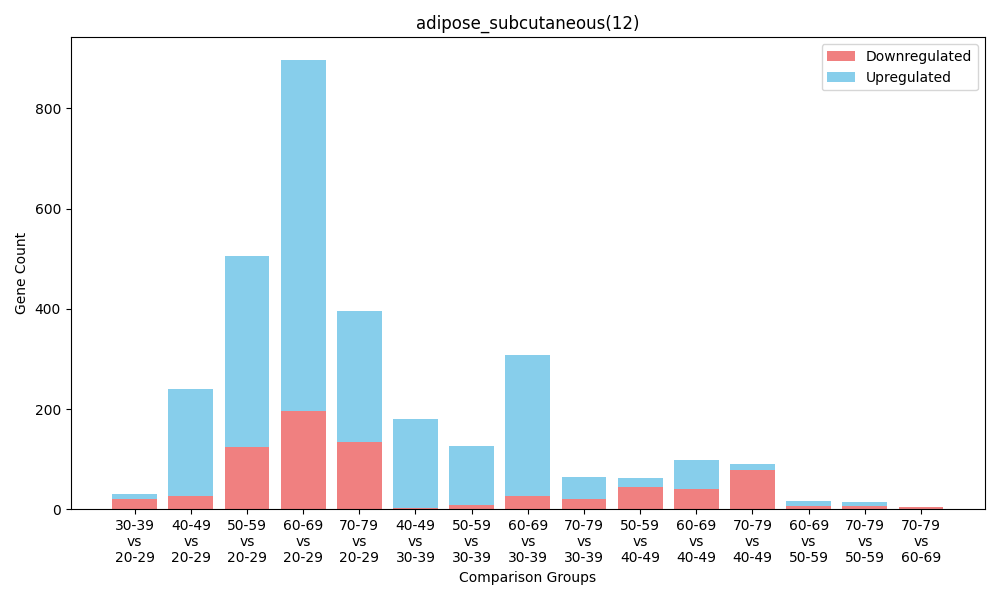
\includegraphics[width=\linewidth]{Clustering_Age_DTHHRDY_Images/adipose_subcutaneous.png}
        \caption{Clustering of adipose subcutaneous tissue tpms}
    \end{subfigure}
    \hfill
    \begin{subfigure}{0.3\linewidth}
        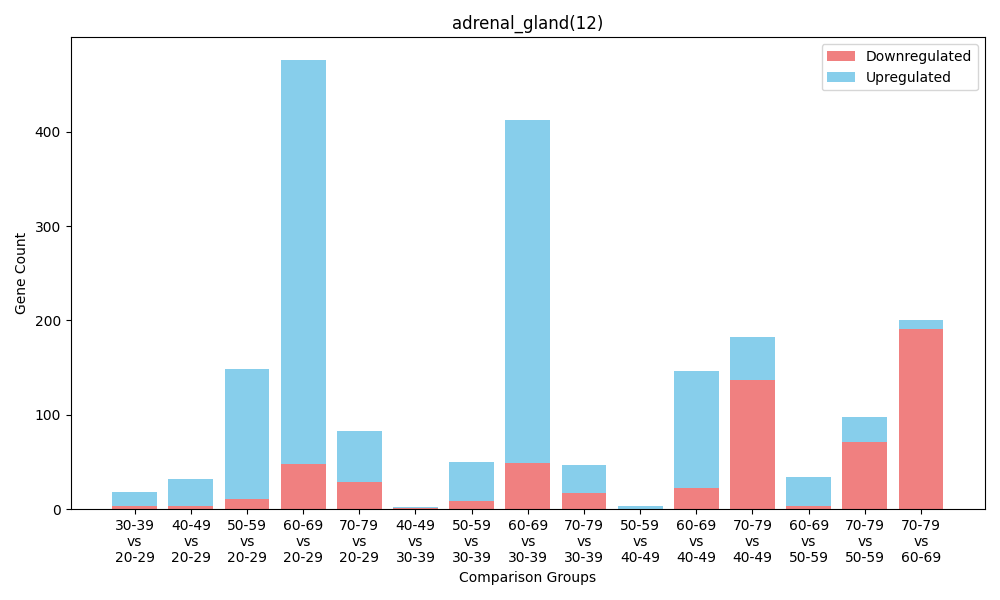
\includegraphics[width=\linewidth]{Clustering_Age_DTHHRDY_Images/adrenal_gland.png}
        \caption{Clustering of adrenal gland tissue tpms}
    \end{subfigure}
    \hfill
    \begin{subfigure}{0.3\linewidth}
        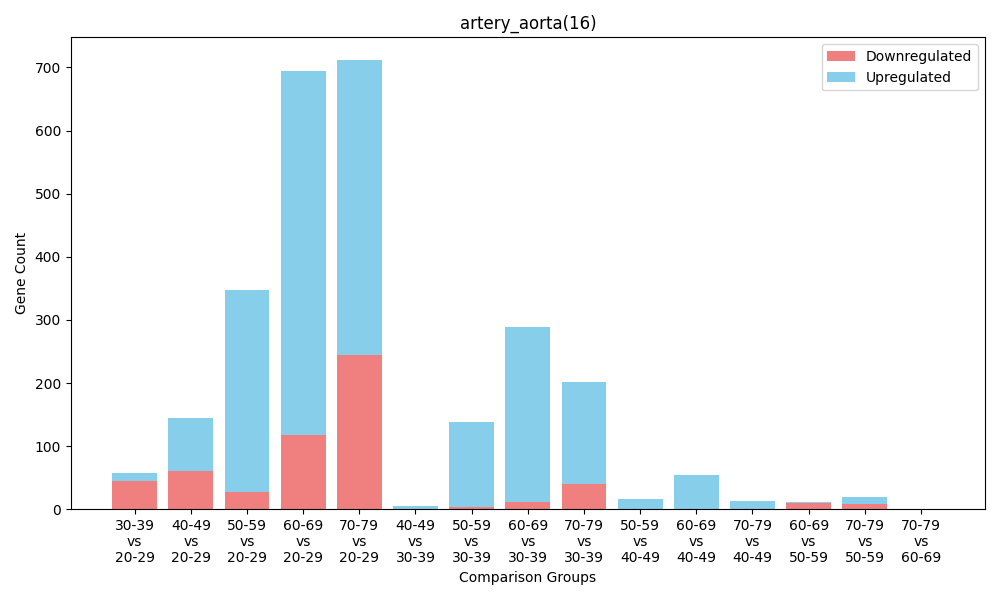
\includegraphics[width=\linewidth]{Clustering_Age_DTHHRDY_Images/artery_aorta.png}
        \caption{Clustering of artery aorta tissue tpms}
    \end{subfigure}

    \vspace{1em}

    % Second row of images
    \begin{subfigure}{0.3\linewidth}
        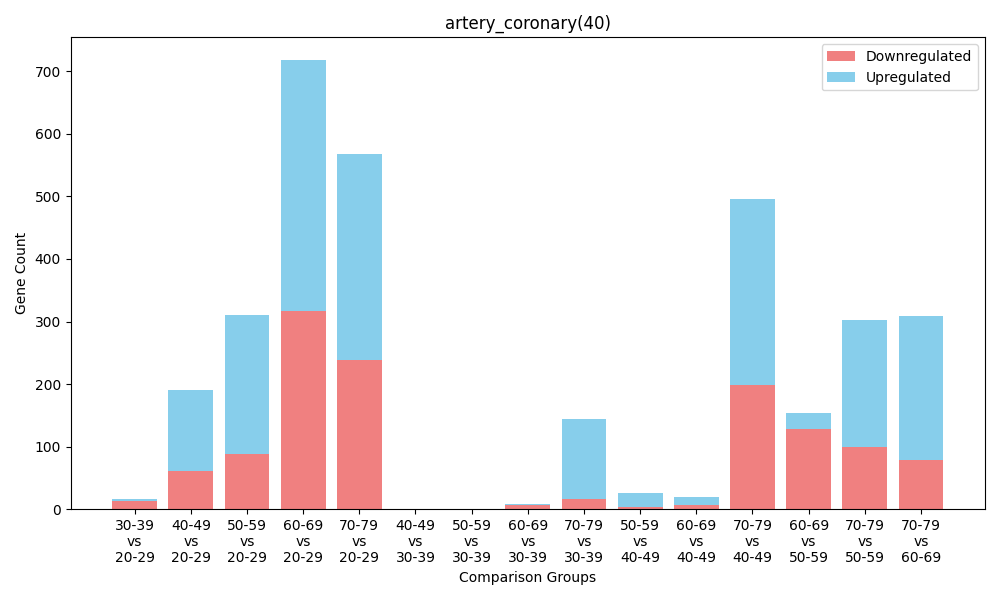
\includegraphics[width=\linewidth]{Clustering_Age_DTHHRDY_Images/artery_coronary.png}
        \caption{Clustering of artery coronary tissue tpms}
    \end{subfigure}
    \hfill
    \begin{subfigure}{0.3\linewidth}
        \includegraphics[width=\linewidth]{Clustering_Age_DTHHRDY_Images/brain_caudate_basal_ganglia.png}
        \caption{Clustering of brain caudate basal tissue tpms}
    \end{subfigure}
    \hfill
    \begin{subfigure}{0.3\linewidth}
        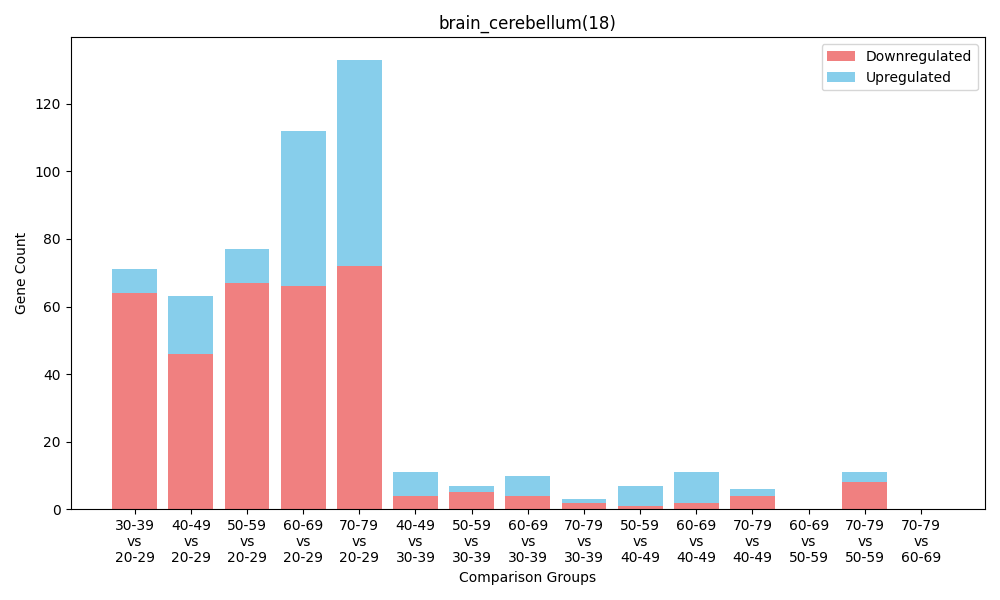
\includegraphics[width=\linewidth]{Clustering_Age_DTHHRDY_Images/brain_cerebellum.png}
        \caption{Clustering of brain cerebellum tissue tpms}
    \end{subfigure}

    \vspace{1em}

    % Third row of images
    \begin{subfigure}{0.3\linewidth}
        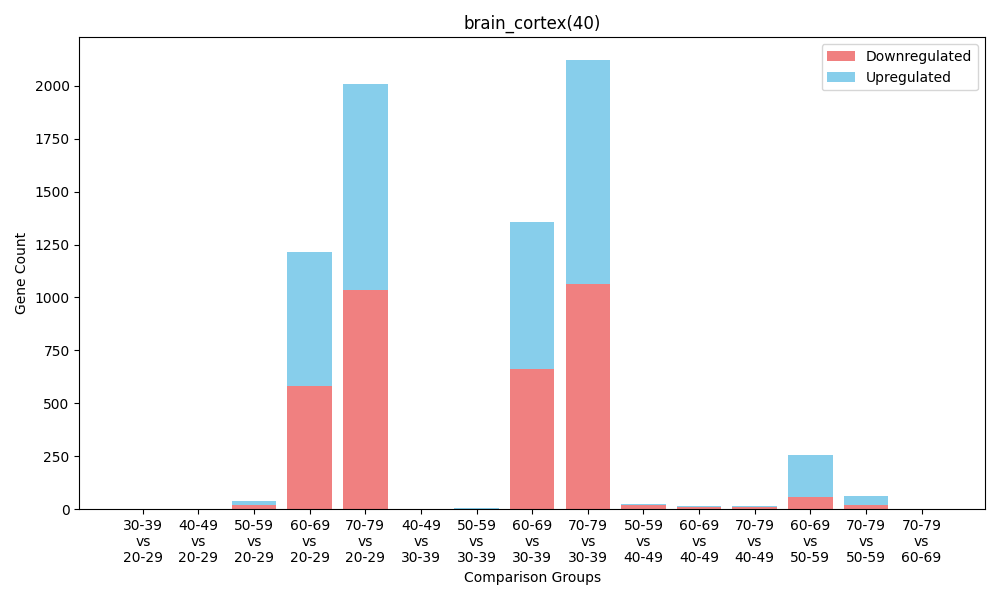
\includegraphics[width=\linewidth]{Clustering_Age_DTHHRDY_Images/brain_cortex.png}
        \caption{Clustering of brain cortex tissue tpms}
    \end{subfigure}
    \hfill
    \begin{subfigure}{0.3\linewidth}
        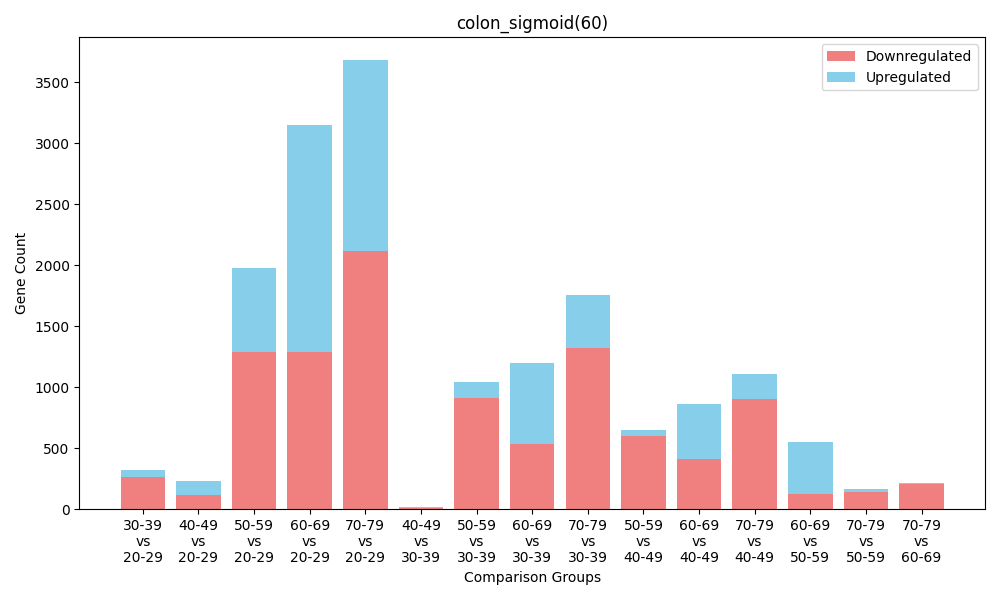
\includegraphics[width=\linewidth]{Clustering_Age_DTHHRDY_Images/colon_sigmoid.png}
        \caption{Clustering of colon sigmoid tissue tpms}
    \end{subfigure}
    \hfill
    \begin{subfigure}{0.3\linewidth}
        \includegraphics[width=\linewidth]{Clustering_Age_DTHHRDY_Images/colon_transverse.png}
        \caption{Clustering of colon transverse tissue tpms}
    \end{subfigure}

    \vspace{1em}

    % Fourth row of images
    \begin{subfigure}{0.3\linewidth}
        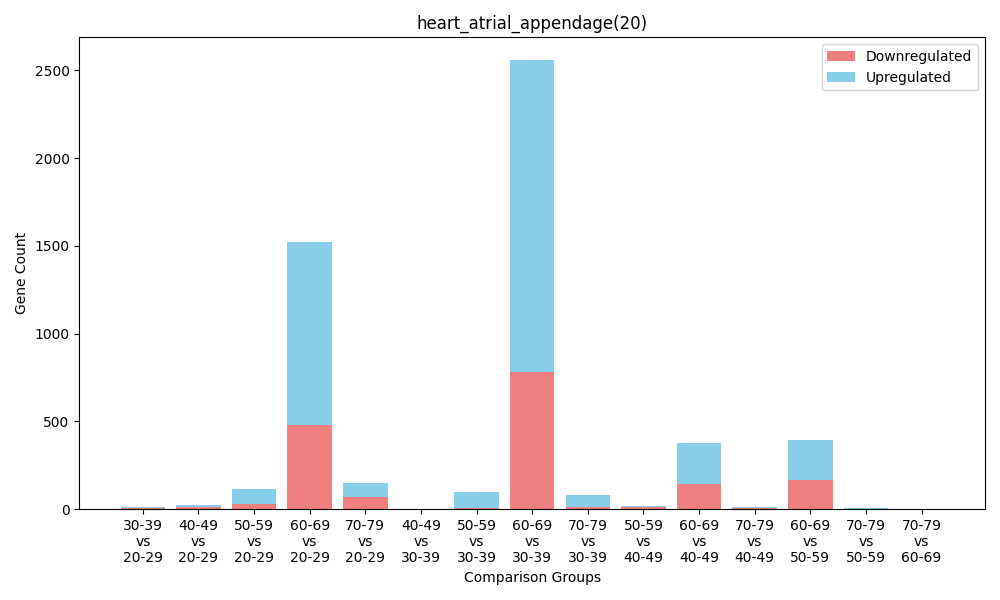
\includegraphics[width=\linewidth]{Clustering_Age_DTHHRDY_Images/heart_atrial_appendage.png}
        \caption{Clustering of heart atrial appendage tissue tpms}
    \end{subfigure}
    \hfill
    \begin{subfigure}{0.3\linewidth}
        \includegraphics[width=\linewidth]{Clustering_Age_DTHHRDY_Images/heart_left_ventricle.png}
        \caption{Clustering of heart left ventricle tissue tpms}
    \end{subfigure}
    \hfill
    \begin{subfigure}{0.3\linewidth}
        \includegraphics[width=\linewidth]{Clustering_Age_DTHHRDY_Images/kidney_cortex.png}
        \caption{Clustering of kidney cortex tissue tpms}
    \end{subfigure}

    \vspace{1em}

    % Fifth row of images
    \begin{subfigure}{0.3\linewidth}
        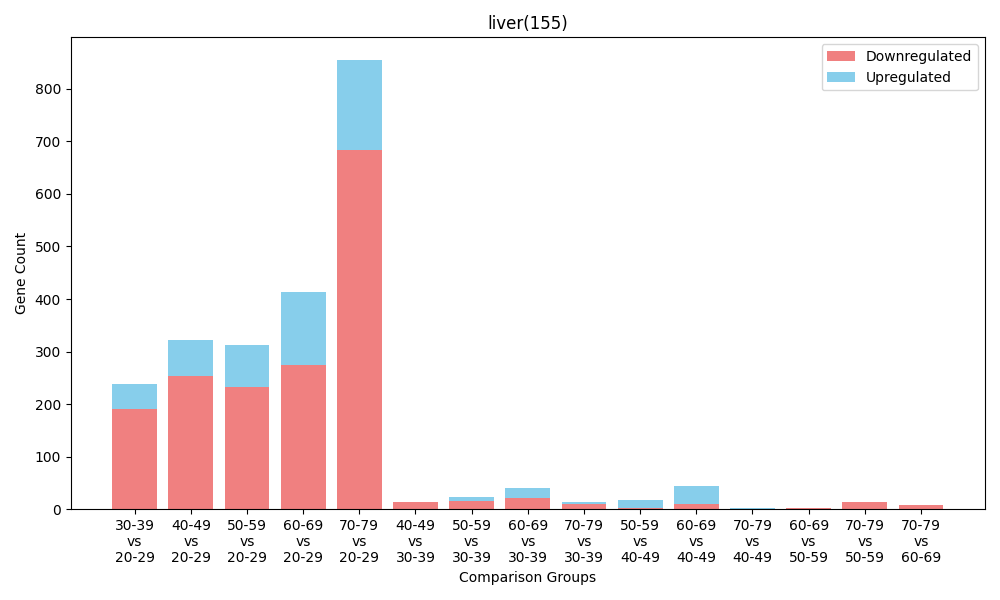
\includegraphics[width=\linewidth]{Clustering_Age_DTHHRDY_Images/liver.png}
        \caption{Clustering of liver tissue tpms}
    \end{subfigure}
    \hfill
    \begin{subfigure}{0.3\linewidth}
        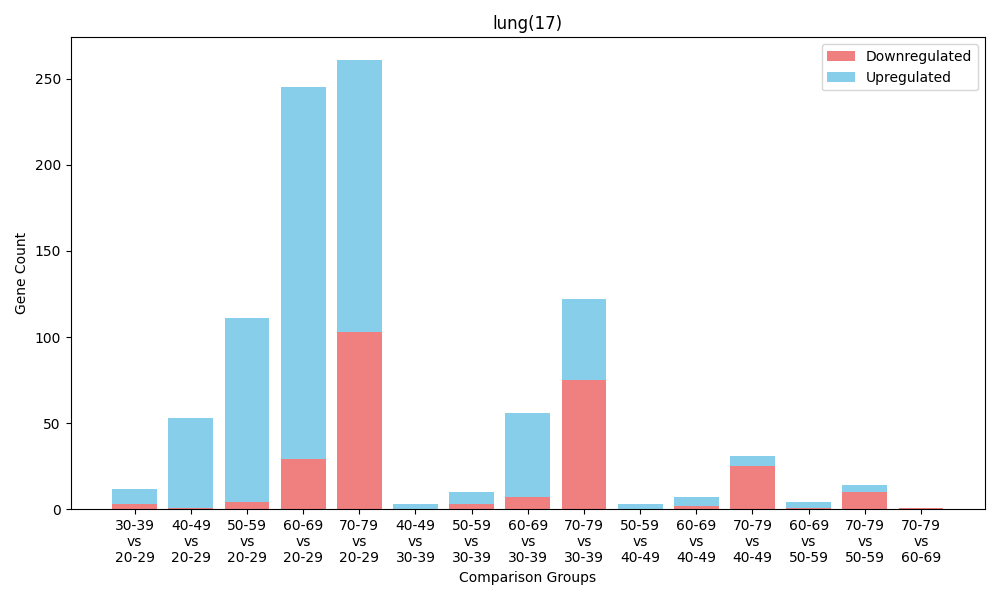
\includegraphics[width=\linewidth]{Clustering_Age_DTHHRDY_Images/lung.png}
        \caption{Clustering of lung tissue tpms}
    \end{subfigure}
    \hfill
    \begin{subfigure}{0.3\linewidth}
        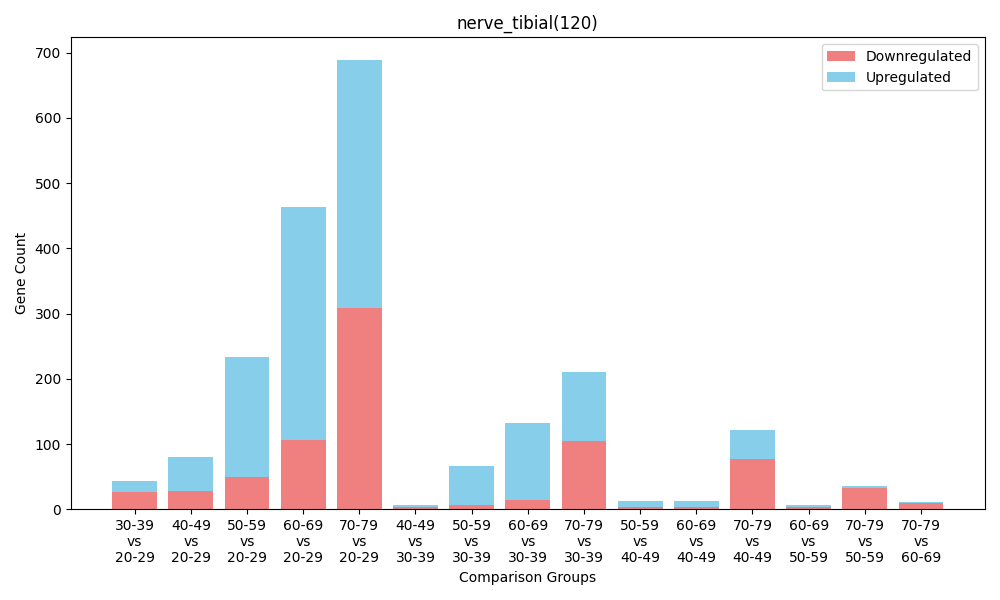
\includegraphics[width=\linewidth]{Clustering_Age_DTHHRDY_Images/nerve_tibial.png}
        \caption{Clustering of nerve tibial tissue tpms}
    \end{subfigure}

    \caption{Part 1: Plots 1 to 15 of T-SNE plots for individual organs}
    \label{fig:T-SNE plots for individual organs_part1}
\end{figure}

    \begin{figure}[H]
    \ContinuedFloat
    \centering
    %Sixth row of images
    \begin{subfigure}{0.3\linewidth}
        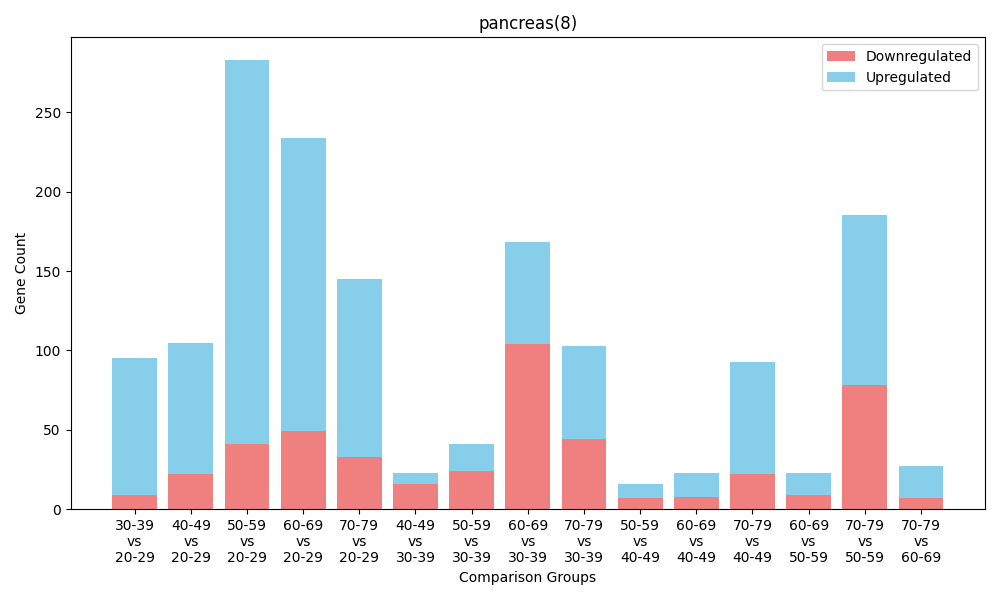
\includegraphics[width=\linewidth]{Clustering_Age_DTHHRDY_Images/pancreas.png}
        \caption{Clustering of pancreas tissue tpms}
    \end{subfigure}
    \hfill
    \begin{subfigure}{0.3\linewidth}
        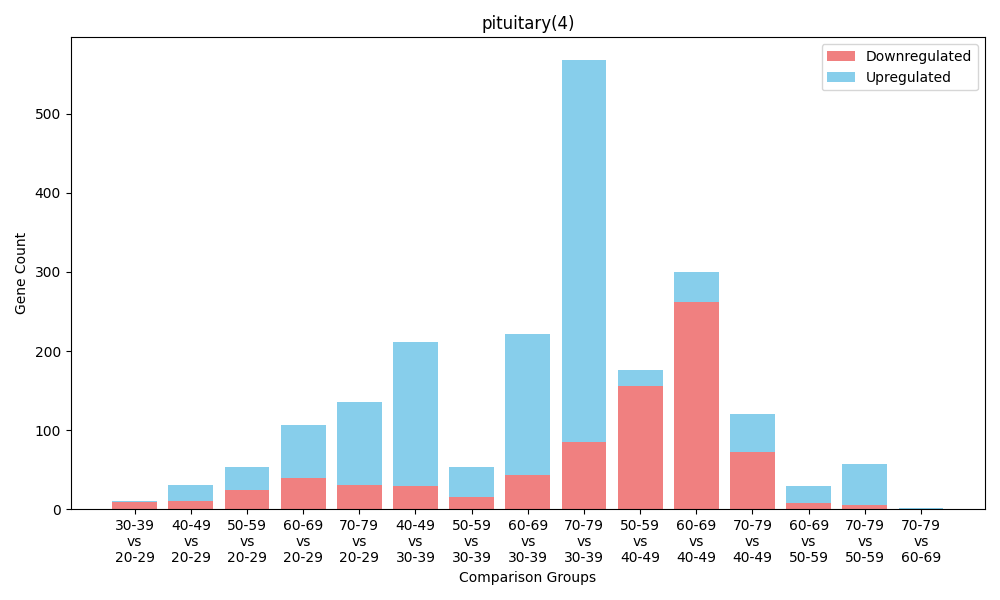
\includegraphics[width=\linewidth]{Clustering_Age_DTHHRDY_Images/pituitary.png}
        \caption{Clustering of pituitary tissue tpms}
    \end{subfigure}
    \hfill
    \begin{subfigure}{0.3\linewidth}
        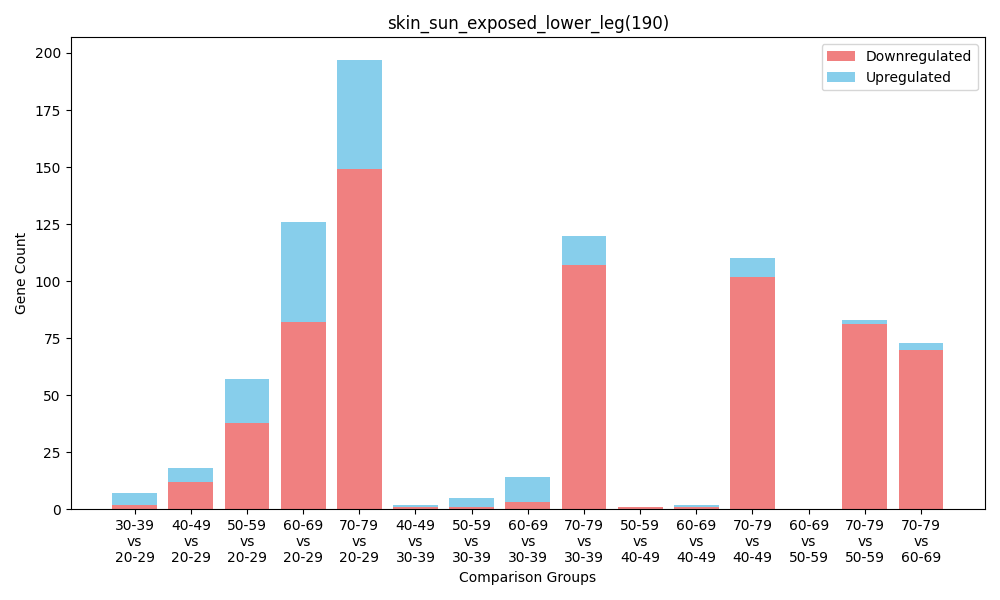
\includegraphics[width=\linewidth]{Clustering_Age_DTHHRDY_Images/skin_sun_exposed_lower_leg.png}
        \caption{Clustering of skin(sun-exposed lower leg) tissue tpms}
    \end{subfigure}

    \vspace{1em}

    %Seventh row of images
    \begin{subfigure}{0.3\linewidth}
        \includegraphics[width=\linewidth]{Clustering_Age_DTHHRDY_Images/stomach.png}
        \caption{Clustering of stomach tissue tpms}
    \end{subfigure}
    \hfill
    \begin{subfigure}{0.3\linewidth}
        \includegraphics[width=\linewidth]{Clustering_Age_DTHHRDY_Images/thyroid.png}
        \caption{Clustering of thyroid tissue tpms}
    \end{subfigure}
    \hfill

   \caption{Part 2: Plots 16 to 20 of T-SNE plots for individual organs}
    \label{fig:T-SNE plots for individual organs_part2}
\end{figure}

We conducted the test-train split multiple times(20+) across several random configurations. For each iteration of the experiment, we performed a conditional probability analysis and averaged the probabilities obtained. This approach was employed to mitigate the influence of randomness on the results, thereby enhancing the reliability of our findings.

\section{Results}

When plotted each subject's minimum observed age gap across all tissue samples (11-19 tissues) in a scatterplot, it appeared to conform to a normal distribution. At the two extremes of this distribution, we identified groups referred to as \textbf{\emph{extreme negative agers}} and \textbf{\emph{extreme positive agers}}, defined as those falling below $(\textbf{\textit{mean} - \textit{stddev}})$ and above $(\textbf{\textit{mean} + \textit{stddev}})$, respectively. Conversely, individuals situated near the center of the distribution, approximately within $(\pm 0.5 \times \textit{stddev})$ around the mean, were categorized as \textbf{\emph{average agers}}.\\

From the minimum age gap of each individual, which we consider as a baseline marker of health, we obtained the following results Table \ref{tab:conditional_probabilities_of_DTHHRDY} \textit{(noting that these findings were derived using Lasso regression)} :\\

\begin{table}[h!]
    \centering
    \caption{Conditional Probabilities and Risk Ratios for Different DTHHRDY Values}
    \begin{tabular}{|c|c|c|c|c|}
        \hline
       \textbf{DTHHRDY} & \textbf{Extreme Positive Agers} & \textbf{Extreme Negative Agers} & \textbf{Average Agers} & \textbf{Overall} (p) \\
        \hline
        0 & $0.3679$ & $0.5980$ & $0.598$ & $0.4570$ \\
        \hline
        1 & $0.0363$ & $0.0734$ & $0.073$ & $0.0591$ \\
        \hline
        2 & $0.3235$ & $0.1995$ & $0.200$ & $0.3001$ \\
        \hline
        3 & $0.0709$ & $0.0269$ & $0.027$ & $0.0572$ \\
        \hline
        4 & $0.2013$ & $0.1022$ & $0.102$ & $0.1266$ \\
        \hline
    \end{tabular}
    \label{tab:conditional_probabilities_of_DTHHRDY}
\end{table}

\noindent The following observations were made based on the calculated conditional probabilities:

\begin{itemize}
    \item \textbf{DTHHRDY=0}:
    \begin{itemize}
        \item Extreme negative agers are 1.625 times more likely to have died with DTHHRDY=0 compared to extreme positive agers.
        \item Extreme negative agers are 1.308 times more likely to have died with DTHHRDY=0 compared to all other groups.
        \item Average agers are 1.167 times more likely to have died with DTHHRDY=0 compared to extreme positive agers.
        \item Extreme negative agers are 1.393 times more likely to have died with DTHHRDY=0 compared to average agers.
    \end{itemize}

    \item \textbf{DTHHRDY=1}:
    \begin{itemize}
        \item Extreme negative agers are 2.019 times more likely to have died with DTHHRDY=1 compared to extreme positive agers.
        \item Extreme negative agers are 1.241 times more likely to have died with DTHHRDY=1 compared to all other groups.
        \item Average agers are 1.600 times more likely to have died with DTHHRDY=1 compared to extreme positive agers.
        \item Extreme negative agers are 1.262 times more likely to have died with DTHHRDY=1 compared to average agers.
    \end{itemize}

    \item \textbf{DTHHRDY=2}:
    \begin{itemize}
        \item Extreme positive agers are 1.621 times more likely to have died with DTHHRDY=2 compared to extreme negative agers.
        \item Extreme positive agers are 1.078 times more likely to have died with DTHHRDY=2 compared to all other groups.
        \item Average agers are 1.074 times more likely to have died with DTHHRDY=2 compared to extreme positive agers.
        \item Average agers are 1.742 times more likely to have died with DTHHRDY=2 compared to extreme negative agers.
    \end{itemize}

    \item \textbf{DTHHRDY=3}:
    \begin{itemize}
        \item Extreme positive agers are 2.635 times more likely to have died with DTHHRDY=3 compared to extreme negative agers.
        \item Extreme positive agers are 1.240 times more likely to have died with DTHHRDY=3 compared to all other groups.
        \item Extreme positive agers are 1.128 times more likely to have died with DTHHRDY=3 compared to average agers.
        \item Average agers are 2.337 times more likely to have died with DTHHRDY=3 compared to extreme negative agers.
    \end{itemize}

    \item \textbf{DTHHRDY=4}:
    \begin{itemize}
        \item Extreme positive agers are 1.970 times more likely to have died with DTHHRDY=4 compared to extreme negative agers.
        \item Extreme positive agers are 1.590 times more likely to have died with DTHHRDY=4 compared to all other groups.
        \item Extreme positive agers are 1.972 times more likely to have died with DTHHRDY=4 compared to average agers.
        \item Extreme negative agers are 1.001 times more likely to have died with DTHHRDY=4 compared to average agers.
    \end{itemize}
\end{itemize}


\section{Discussion}

\begin{enumerate}
    \item The tissues are distinguishable based solely on their 56,000 TPM values, as indicated by the t-SNE analysis. This suggests that each organ possesses a unique transcriptomic profile.

    \item There exists a linear correspondence between the predicted age and actual age, as evidenced by the LOWESS regression analysis presented in the graph. This observation indicates a correlation between gene TPM values and age, suggesting that gene expression levels can be utilized for age prediction. The $R^{2}$ values ranging from 0.4 to 0.5 for most organs imply that approximately 50\% of the variance in the predicted age can be explained by the variance in gene TPMs.

    \item We calculated the conditional probability of each DTHHRDY value for each organ; however, it is important to note that these probabilities do not imply causation, as the specific organ responsible for the cause of death remains unknown. Additionally, the organs that exhibited unexpected results also demonstrated poorer fits in the regression model, as indicated by both the graphical representation and the R² values.

     \item Subsequently, we computed the conditional probability of each DTHHRDY value's distribution within the ranges designated for extreme negative agers, extreme positive agers, and average agers. Including the poorly fitting organs mentioned above in the calculation of the total subjects' minimum or average age tends to yield similarly unexpected results.
\end{enumerate}

\bibliographystyle{plainnat}
\bibliography{bibliography}

\end{document}
